\documentclass[conference]{IEEEtran}
\IEEEoverridecommandlockouts

\usepackage{cite}
\usepackage{amsmath,amssymb,amsfonts}
\usepackage{algorithmic}
\usepackage{graphicx}
\usepackage{textcomp}
\usepackage{xcolor}
\usepackage{hyperref}
\usepackage{booktabs}
\usepackage{array}
\usepackage{url}
\usepackage{tikz}
\usetikzlibrary{arrows.meta,positioning,shapes.geometric}

\hypersetup{
    colorlinks=true,
    linkcolor=blue,
    citecolor=blue,
    urlcolor=blue
}

\def\BibTeX{{\rm B\kern-.05em{\sc i\kern-.025em b}\kern-.08em
    T\kern-.1667em\lower.7ex\hbox{E}\kern-.125emX}}

\begin{document}

\title{Carbon Footprint Prediction System Using Big Data Infrastructure and Machine Learning: A Scalable AI-Driven Approach for Sustainability}

\author{
    \IEEEauthorblockN{Mehmet Daşkaya}
    \IEEEauthorblockA{
        \textit{Department of Big Data Analytics and Management} \\
        \textit{Bahçeşehir University} \\
        Istanbul, Turkiye \\
        \textit 2003445 \\
        mehmet.daskaya@bahcesehir.edu.tr
    }
}

\maketitle

\begin{abstract}
Climate change and greenhouse gas emissions represent one of the most critical challenges of the 21st century. Accurate prediction of carbon footprints at scale is essential for formulating effective sustainability policies and enabling real-time environmental monitoring. This proposal presents a scalable Big Data-driven system for predicting carbon footprints across multiple sectors — including transportation, energy production, and industry — by integrating Apache Spark for distributed processing, MongoDB for flexible NoSQL storage, Apache Kafka for real-time data ingestion, and a machine learning pipeline built on gradient boosting and LSTM-based deep learning models. The system ingests data from publicly available sources such as the EDGAR global emissions database and the Carbon Monitor dataset, enabling near-real-time analysis. A Next.js-based interactive dashboard will visualize emission trends and model predictions. The proposed architecture is designed to be modular, horizontally scalable, and aligned with the UN Sustainable Development Goals.
\end{abstract}

\begin{IEEEkeywords}
carbon footprint, big data, Apache Spark, MongoDB, machine learning, LSTM, sustainability, distributed computing, Apache Kafka, emissions prediction
\end{IEEEkeywords}

% -------------------------------------------------------
\section{Problem Definition}

\subsection{Motivation and Real-World Significance}
Global carbon dioxide (CO\textsubscript{2}) emissions reached approximately 36.8 billion tonnes in 2023, with the energy, transportation, and industrial sectors accounting for the vast majority of contributions \cite{carbonmonitor2020}. Despite growing international commitments under the Paris Agreement, the gap between emission reduction targets and actual progress remains substantial. Accurate, timely, and spatially resolved carbon footprint data is a prerequisite for evidence-based climate policy, corporate sustainability reporting, and urban planning.

Traditional emissions reporting is conducted on an annual basis, with lags of one year or more \cite{edgar2021}. This temporal coarseness prevents policymakers and organizations from responding to sudden emission spikes, seasonal trends, or the effects of policy interventions in near-real-time. Furthermore, existing solutions are often domain-specific, non-scalable, and lack integration with modern AI techniques.

\subsection{Problem Statement}
The core problem addressed in this project is: \textit{how can we build a scalable, near-real-time system that ingests heterogeneous multi-source emission data, processes it efficiently using distributed computing, and accurately predicts carbon footprints at sector and regional levels using machine learning?}

\subsection{Why Big Data and AI are Required}
The datasets involved — including global gridded emissions at 0.1° resolution, hourly electricity generation records, and real-time traffic indices — are inherently large-scale, multi-modal, and high-velocity. Classical relational databases and single-node processing pipelines cannot handle such data volumes efficiently. A Big Data infrastructure (Spark, Kafka, distributed storage) is necessary for ingestion and processing at scale, while AI/ML models are needed to capture the non-linear temporal and spatial patterns that govern emissions dynamics.

% -------------------------------------------------------
\section{Dataset Description \& Visualization}

\subsection{Primary Datasets}

\subsubsection{EDGAR — Emission Database for Global Atmospheric Research}
Developed by the European Commission Joint Research Centre (JRC), EDGAR provides global anthropogenic greenhouse-gas inventories with gridded products at up to 0.1$^{\circ}$ spatial resolution and long historical coverage beginning in 1970 \cite{edgar2021}. For this project, EDGAR is the most suitable source for large-scale historical baseline modeling because it offers harmonized sector definitions, country-level aggregation, and spatial grids that support both sectoral forecasting and map-based visualization. The dataset family is distributed through downloadable archives and tabular products and is large enough to justify distributed storage and Spark-based batch processing.
\begin{center}
\url{https://edgar.jrc.ec.europa.eu/}
\end{center}

\subsubsection{Carbon Monitor — Near-Real-Time Daily CO\textsubscript{2} Emissions}
Carbon Monitor provides near-real-time daily CO\textsubscript{2} emission estimates derived from high-frequency activity indicators such as power generation, ground transport, industry, residential activity, aviation, and shipping \cite{carbonmonitor2020}. It is well-suited for the streaming branch of the proposed architecture because it complements EDGAR's historical inventory data with a much finer temporal granularity. In this proposal, Carbon Monitor is treated as a continuously refreshed daily input dataset rather than as an official transactional API source, making scheduled file ingestion a more realistic implementation choice.
\begin{center}
\url{https://carbonmonitor.org/}
\end{center}

\subsubsection{Kaggle — Individual Carbon Footprint Dataset}
This Kaggle dataset provides individual-level lifestyle records related to transportation habits, home energy use, diet, and consumption patterns \cite{kaggle_carbon}. It is suitable as an \textit{auxiliary} dataset for a behavioral classification subtask (low/medium/high personal footprint), but it should not be presented as a substitute for measured national or sectoral emissions inventories. Accordingly, its role in this project is limited to demonstrating user-level classification and dashboard personalization rather than core macro-scale forecasting.
\begin{center}
\url{https://www.kaggle.com/datasets/dumanmesut/individual-carbon-footprint-calculation}
\end{center}

\subsubsection{CO\textsubscript{2} Emissions from Vehicles — Canadian Government Open Data}
This transportation dataset, mirrored on Kaggle and originally sourced from the Government of Canada's fuel-consumption ratings data, contains structured vehicle attributes such as engine size, cylinders, transmission, fuel type, fuel consumption, and CO\textsubscript{2} emissions \cite{vehicles_co2}. It is appropriate for supervised regression experiments and for validating feature-engineering choices in the transportation domain. However, because it represents certified vehicle-level measurements rather than observed fleet activity, it is best positioned as a complementary transportation dataset rather than the main driver of national-scale forecasting.
\begin{center}
\url{https://www.kaggle.com/datasets/debajyotipodder/co2-emission-by-vehicles}
\end{center}

\subsection{Dataset Summary}
Table~\ref{tab:datasets} summarizes the role and suitability of each dataset in the final design.

\begin{table}[h]
\caption{Dataset Overview}
\label{tab:datasets}
\centering
\scriptsize
\resizebox{\columnwidth}{!}{%
\begin{tabular}{p{1.9cm} p{1.2cm} p{1.2cm} p{1.7cm} p{2.1cm}}
\toprule
\textbf{Dataset} & \textbf{Scale} & \textbf{Format} & \textbf{Primary Role} & \textbf{Suitability} \\
\midrule
EDGAR & Large & Archives/CSV & Historical batch baseline & Excellent for sectoral and spatial modeling \\
Carbon Monitor & Medium & CSV & Near-real-time daily updates & Excellent for streaming and short-horizon forecasting \\
Kaggle Individual & Small & CSV & Behavioral classification demo & Useful only as an auxiliary micro-level task \\
Vehicle CO\textsubscript{2} & Small & CSV & Transport-domain regression & Good for transportation experiments, not national inventories \\
\bottomrule
\end{tabular}
}
\end{table}

\subsection{Dataset Suitability Statement}
The dataset mix is appropriate for the project \textit{if the roles are clearly separated}. EDGAR and Carbon Monitor should remain the core sources for macro-scale emissions forecasting because they provide consistent temporal and sectoral coverage. The Kaggle individual and vehicle datasets strengthen the paper by adding explainable downstream use cases, but they should be framed as supporting datasets for classification and transportation-specific regression rather than as primary evidence for country-level carbon accounting.

\subsection{Exploratory Data Analysis Plan}
Exploratory Data Analysis (EDA) will be conducted using Apache Spark SQL and Python (Pandas, Matplotlib, Seaborn) and will include: (1) temporal trend analysis of daily and annual CO\textsubscript{2} emissions per sector; (2) geographical heatmaps using EDGAR gridded data; (3) correlation analysis between energy consumption features and emission levels; (4) distribution analysis of individual carbon footprint features; and (5) outlier detection across vehicle emission records. All visualizations will be embedded in the Next.js dashboard.

% -------------------------------------------------------
\section{Data Preprocessing}

\subsection{Data Cleaning}
Raw datasets from EDGAR and Carbon Monitor contain missing values, inconsistent country codes, and format heterogeneity (archive/grid files vs. CSV tables). A standardized preprocessing pipeline will be implemented using Apache Spark DataFrames to: (1) normalize gridded and tabular source files into a unified schema; (2) align temporal granularities across datasets (daily, monthly, annual); (3) standardize country and region identifiers using ISO 3166 codes; and (4) remove duplicate records and handle null values through interpolation, median imputation, or forward-fill for time-series data as appropriate.

\subsection{Feature Engineering}
New derived features will be constructed to improve model performance, including: rolling 7-day and 30-day average emissions (temporal smoothing), emission intensity ratios (CO\textsubscript{2} per GDP unit, CO\textsubscript{2} per capita), seasonal indicators (month, quarter, public holiday flags), and lagged emission values for time-series modeling (lag-1, lag-7, lag-30). Categorical variables such as fuel type and emission sector will be encoded using one-hot encoding. Numerical features will be normalized using Min-Max scaling or Z-score standardization depending on the target model.

\subsection{Handling Class Imbalance}
For the classification subtask (individual carbon footprint levels: low, medium, high), SMOTE (Synthetic Minority Over-sampling Technique) will be applied to address class imbalance in the Kaggle individual dataset.

% -------------------------------------------------------
\section{NoSQL Database — MongoDB}

\subsection{Justification for NoSQL}
The heterogeneous nature of the data — ranging from structured tabular records (vehicle emissions) to semi-structured JSON-style sensor readings and nested geographical metadata — makes a document-oriented NoSQL database highly appropriate. MongoDB offers schema flexibility, native support for GeoJSON spatial queries, and a time-series collection type (introduced in MongoDB 5.0) that is optimized for storing and querying high-frequency temporal emission data \cite{mongodb_ts}.

\subsection{Data Modeling Strategy}
Three primary MongoDB collections will be defined:
\begin{itemize}
    \item \textbf{emissions\_timeseries}: Time-series collection storing daily emission records per country and sector, indexed by timestamp and region code.
    \item \textbf{individual\_records}: Document collection for individual carbon footprint records from the Kaggle dataset, including lifestyle features and predicted emission class.
    \item \textbf{vehicle\_records}: Collection of vehicle-level emission records with engine attributes and CO\textsubscript{2} output, supporting geospatial queries by registration region.
\end{itemize}

MongoDB Atlas will be used as the managed cloud deployment, enabling horizontal sharding for large EDGAR datasets and integration with Spark via the MongoDB Connector for Apache Spark.

% -------------------------------------------------------
\section{Big Data Infrastructure}

\subsection{Apache Kafka — Real-Time Data Ingestion}
Apache Kafka will serve as the ingestion layer for near-real-time updates derived from Carbon Monitor's daily releases. A scheduled ingestion service will fetch newly published daily data files, validate schema consistency, and publish standardized emission records to a dedicated topic (\texttt{carbon-emissions-daily}). Multiple Kafka consumers will subscribe to this topic to feed downstream processing and storage pipelines.

\subsection{Apache Spark — Distributed Processing}
Apache Spark will be the central processing engine for all batch and stream processing tasks:
\begin{itemize}
    \item \textbf{Batch processing}: EDGAR and vehicle datasets will be processed as Spark DataFrames, applying preprocessing, feature engineering, and aggregation transformations.
    \item \textbf{Streaming}: Spark Structured Streaming will consume from Kafka topics and compute rolling emission statistics in near-real-time.
    \item \textbf{ML pipeline}: Spark MLlib will be used for baseline model training (Random Forest, Gradient Boosted Trees) on distributed data.
\end{itemize}

\subsection{Distributed File System — HDFS / Cloud Storage}
Raw dataset files (EDGAR NetCDF archives, $\sim$50 GB) will be stored in HDFS or a cloud-equivalent distributed object storage (e.g., AWS S3 or MinIO), partitioned by year and sector for efficient Spark reads.

% -------------------------------------------------------
\section{AI Application}

\subsection{Task Formulation}
Two prediction tasks are defined: (1) \textbf{Regression}: predict continuous daily CO\textsubscript{2} emission values per sector and country; (2) \textbf{Classification}: predict individual carbon footprint level (low/medium/high) based on lifestyle features.

\subsection{Model Selection}

\subsubsection{LSTM (Long Short-Term Memory)}
For the temporal regression task, an LSTM-based deep learning model will be developed using PyTorch. LSTM networks are well-suited for multi-step time-series forecasting, capable of capturing long-range temporal dependencies in daily emission sequences \cite{lstm_energy}. Input sequences of 30 days will be used to predict emission values for the next 7 days (multi-step ahead forecasting).

\subsubsection{Gradient Boosted Trees (XGBoost / LightGBM)}
For both regression and classification tasks, gradient boosting models will serve as strong baselines. These models are interpretable, computationally efficient, and handle mixed feature types well. SHAP (SHapley Additive exPlanations) values will be computed to provide feature importance explanations.

\subsubsection{Spark MLlib — Random Forest}
A distributed Random Forest model via Spark MLlib will be trained on the full EDGAR dataset to enable scalable sector-level emission prediction across all countries simultaneously.

\subsection{Training and Evaluation}
All models will be trained with an 80/10/10 train/validation/test split, using time-based splitting for time-series models to prevent data leakage. Evaluation metrics include Mean Absolute Error (MAE), Root Mean Squared Error (RMSE), and R\textsuperscript{2} for regression tasks; and Accuracy, Precision, Recall, and F1-score for classification. Model performance will be tracked using MLflow for experiment logging.

% -------------------------------------------------------
\section{System Architecture}

\subsection{Overview}
The system follows a layered Lambda Architecture pattern, combining batch and streaming processing paths into a unified serving layer. Fig.~\ref{fig:architecture} illustrates the high-level system design.

\begin{figure*}[t]
\centering
\resizebox{0.9\textwidth}{!}{%
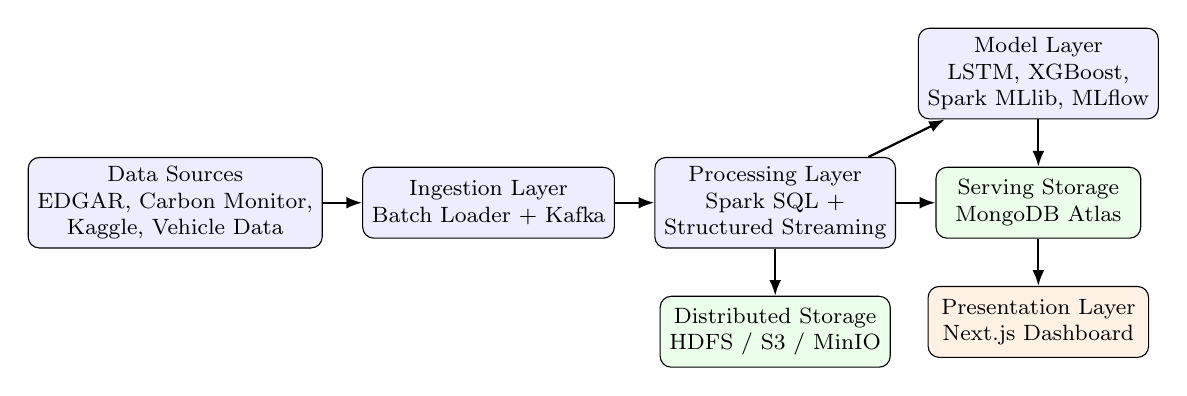
\begin{tikzpicture}[
    font=\footnotesize,
    node distance=6mm and 5mm,
    block/.style={draw, rounded corners, align=center, minimum width=24mm, minimum height=9mm, fill=blue!7},
    store/.style={draw, rounded corners, align=center, minimum width=26mm, minimum height=9mm, fill=green!8},
    app/.style={draw, rounded corners, align=center, minimum width=28mm, minimum height=9mm, fill=orange!10},
    line/.style={-{Latex[length=2mm]}, thick}
]
\node[block] (sources) {Data Sources\\EDGAR, Carbon Monitor,\\Kaggle, Vehicle Data};
\node[block, right=of sources] (ingest) {Ingestion Layer\\Batch Loader + Kafka};
\node[block, right=of ingest] (spark) {Processing Layer\\Spark SQL +\\Structured Streaming};
\node[store, below=of spark] (raw) {Distributed Storage\\HDFS / S3 / MinIO};
\node[store, right=of spark] (mongo) {Serving Storage\\MongoDB Atlas};
\node[block, above=of mongo] (ml) {Model Layer\\LSTM, XGBoost,\\Spark MLlib, MLflow};
\node[app, below=of mongo] (ui) {Presentation Layer\\Next.js Dashboard};

\draw[line] (sources) -- (ingest);
\draw[line] (ingest) -- (spark);
\draw[line] (spark) -- (mongo);
\draw[line] (spark) -- (raw);
\draw[line] (spark) -- (ml);
\draw[line] (ml) -- (mongo);
\draw[line] (mongo) -- (ui);
\end{tikzpicture}%
}
\caption{High-level system architecture of the Carbon Footprint Prediction System.}
\label{fig:architecture}
\end{figure*}

\subsection{Component Description}
The architecture consists of five layers:

\begin{enumerate}
    \item \textbf{Ingestion Layer}: Apache Kafka producers and scheduled loaders collect daily Carbon Monitor releases together with periodic batch downloads from EDGAR, Kaggle, and transportation datasets.
    \item \textbf{Processing Layer}: Apache Spark handles both Structured Streaming (real-time path) and batch DataFrames (historical path). Preprocessing, feature engineering, and model inference are executed here.
    \item \textbf{Storage Layer}: MongoDB stores processed emission records in time-series and document collections. Raw files reside in HDFS/cloud object storage.
    \item \textbf{Model Layer}: Trained LSTM, XGBoost, and Spark MLlib models perform inference. MLflow manages model versioning and experiment tracking.
    \item \textbf{Presentation Layer}: A Next.js web application with React components provides interactive dashboards for emission trend visualization, regional comparison, and real-time prediction outputs. MongoDB Atlas Data API serves data to the frontend.
\end{enumerate}

\subsection{Data Flow Summary}
Raw emission data arrives via Kafka or batch ingestion → Spark processes and transforms the data → cleaned records are persisted in MongoDB → ML models generate predictions → Next.js dashboard renders visualizations and forecasts for end users.

% -------------------------------------------------------
\section{Innovation and Originality}

This project distinguishes itself from existing work in several ways. First, it integrates \textit{multiple heterogeneous emission datasets} (global gridded, national daily, individual-level, and vehicle-level) into a unified prediction pipeline, enabling cross-scale analysis. Second, the combination of LSTM-based temporal forecasting with SHAP-based explainability bridges predictive performance and interpretability — a gap frequently noted in AI sustainability applications. Third, the use of MongoDB time-series collections with Apache Spark streaming creates a production-grade, horizontally scalable architecture suitable for deployment beyond academic settings. Finally, the Next.js interactive dashboard makes model outputs accessible to non-technical stakeholders, directly supporting policy communication and public sustainability awareness.

% -------------------------------------------------------
\section{Conclusion}

This proposal outlines a comprehensive Big Data and AI system for carbon footprint prediction, addressing the critical need for scalable, real-time emissions monitoring. By leveraging Apache Kafka for ingestion, Apache Spark for distributed processing, MongoDB for flexible storage, and LSTM/XGBoost models for prediction, the system is designed to deliver accurate and actionable emissions insights. The proposed Next.js dashboard further ensures that results are accessible to a broad audience. This work directly contributes to UN Sustainable Development Goal 13 (Climate Action) by enabling data-driven decision-making for emission reduction.

% -------------------------------------------------------
\begin{thebibliography}{00}

\bibitem{carbonmonitor2020}
Z. Liu \textit{et al.}, ``Carbon Monitor, a near-real-time daily dataset of global CO\textsubscript{2} emission from fossil fuel and cement production,'' \textit{Scientific Data}, vol. 7, no. 1, p. 392, 2020. [Online]. Available: \url{https://doi.org/10.1038/s41597-020-00708-7}

\bibitem{edgar2021}
M. Crippa \textit{et al.}, ``EDGAR: Emissions Database for Global Atmospheric Research,'' European Commission, Joint Research Centre (JRC), dataset portal, accessed Apr. 30, 2026. [Online]. Available: \url{https://edgar.jrc.ec.europa.eu/}

\bibitem{kaggle_carbon}
M. Duman, ``Individual Carbon Footprint Calculation,'' Kaggle Dataset, accessed Apr. 30, 2026. [Online]. Available: \url{https://www.kaggle.com/datasets/dumanmesut/individual-carbon-footprint-calculation}

\bibitem{vehicles_co2}
Government of Canada, ``Fuel Consumption Ratings,'' Open Government Portal; mirrored as ``CO2 Emission by Vehicles'' on Kaggle, accessed Apr. 30, 2026. [Online]. Available: \url{https://www.kaggle.com/datasets/debajyotipodder/co2-emission-by-vehicles}

\bibitem{mongodb_ts}
MongoDB, Inc., ``Time Series Collections,'' MongoDB Documentation, accessed Apr. 30, 2026. [Online]. Available: \url{https://www.mongodb.com/docs/manual/core/timeseries-collections/}

\bibitem{lstm_energy}
H. Shi, M. Xu, and R. Li, ``Deep Learning for Household Load Forecasting — A Novel Pooling Deep RNN,'' \textit{IEEE Transactions on Smart Grid}, vol. 9, no. 5, pp. 5271--5280, 2018. \url{https://doi.org/10.1109/TSG.2017.2686238}

\bibitem{graced2022}
D. Zheng \textit{et al.}, ``Near-real-time global gridded daily CO\textsubscript{2} emissions 2021,'' \textit{The Innovation}, vol. 4, no. 1, 2023. [Online]. Available: \url{https://doi.org/10.1016/j.xinn.2022.100350}

\bibitem{cities_co2}
F.-M. Bréon \textit{et al.}, ``A global dataset of CO\textsubscript{2} emissions and ancillary data related to emissions for 343 cities,'' \textit{Scientific Data}, vol. 6, no. 1, p. 180280, 2019. [Online]. Available: \url{https://doi.org/10.1038/sdata.2018.280}

\end{thebibliography}

\end{document}